\documentclass[ % ドキュメントクラス
  uplatex,%upLaTeXを使う
  a5paper,%A5サイズにする
  papersize%紙のサイズがデフォルトと違う場合、PDFにうまく伝える
]{jsbook}

%% フォント関連
%\usepackage[T1]{fontenc} % フォントでT1を使うこと
%\usepackage{textcomp} % フォントでTS1を使うこと
%\usepackage[utf8]{inputenc} % ファイルがUTF8であること
%\usepackage{newpxtext,newpxmath} % ローマンと数式の字体をPalatinoに基づいた新PXフォントで
%\usepackage{zi4}%等幅フォントをInconsolataで
%\usepackage[multi,deluxe,jis2004]{otf}
%\usepackage[prefernoncjk]{pxcjkcat} % なるべく「半角」扱いで。
%\cjkcategory{sym18}{cjk} % sym18 (U+25A0 - U+25FF Geometric Shapes) を和文文字あつかい
%\renewcommand{\bfdefault}{bx}

% 数式など
\usepackage{amsmath}
\usepackage{physics}

%% 図表など
% 図の読みこみのために
\usepackage[dvipdfmx, hiresbb]{graphicx, xcolor}
\usepackage{booktabs} % 表の横罫線
\usepackage{lscape}  % 表などを90度回転させる
\usepackage{here}

%罫線
\makeatletter
  \def\vhrulefill#1{\leavevmode\leaders\hrule\@height#1\hfill \kern\z@}
\makeatother
%URL https://latex.org/forum/viewtopic.php?t=8117

%% 囲み枠
\usepackage{tcolorbox}
\tcbuselibrary{breakable} % ページをまたいで分割できるように
\tcbuselibrary{skins} % さまざまな skin を準備
\tcbuselibrary{theorems} % 定理環境

% 枠の定義
\newtcolorbox{summary}{
  sharp corners, % 角を丸くしない
  boxrule=0pt, % ボックスの罫線なし
  colback=green!20!white, % ボックスの背景色
}

\newtcolorbox{column}{
  breakable,
  sharp corners, % 角を丸くしない
  boxrule=0pt, % ボックスの罫線なし
  colback=blue!20!white, % ボックスの背景色
}

\newtcolorbox{code}{
  breakable,
  sharp corners, % 角を丸くしない
  boxrule=0pt, % ボックスの罫線なし
  colback=black!20!white, % ボックスの背景色
}

\definecolor{safecolor}{rgb}{0.2, 0.4, 0.8}

\newtcolorbox{example}[2][]%%%〇〇の定理
{enhanced,%%%tikzを用いた記法の処理
left=22pt,right=22pt,%%%box内左右の余白
fonttitle=\gtfamily\bfseries,%%%タイトルのフォント指定
coltitle=white,%%%タイトルの文字の色
colbacktitle=blue!50!black,%%%タイトルの背景の色
attach boxed title to top left={},%%%タイトルを左寄せに、少し微調整
boxed title style={skin=enhancedfirst jigsaw,arc=1mm,bottom=0mm,boxrule=0mm},%%%タイトルボックスの装飾
boxrule=0.5pt,%%%枠線の太さ
colback=safecolor!5!,%%%本文の背景色
colframe=safecolor,%%%本文の枠の色
sharp corners=northwest,%%%左上の角の調整
drop fuzzy shadow,%%%影をつける
breakable,%%%ページマタギOK
title=\vspace{3mm}#2,%%%タイトルは直接入力
arc=1mm,%弧
#1}%
%上記までプリアンブル

\newtcolorbox{note}[1]{
  breakable, % ページをまたいでボックスを分割
  before skip=20pt plus 2pt minus 2pt, % ボックスの前の空き
  after skip=20pt plus 2pt minus 2pt, % ボックスの後の空き
  boxrule=0.4pt, % ボックスの罫線の太さ
  colframe=black!95, % フレームの色
  colback=white!95, % ボックスの背景色
  fonttitle=\gtfamily\bfseries, % タイトルのフォント
  title=#1 % タイトルのテキスト
}

% 参考情報を出力する命令を作る
\newtcbox{mysbox}{ % box を作る命令
  boxrule=0.4pt, % ボックスの罫線の太さ
  colframe=black, % フレームの色
  colback=black!10, % ボックスの背景色
  top=0mm,
  bottom=0mm,
  left=0mm,
  right=0mm,
  on line, arc=0.5mm}
\newcommand{\sanko}[1]{%
  \begin{itemize}
    \item[\mysbox{\small\gtfamily 参考}] #1
  \end{itemize}
}

% エピグラフ
\usepackage{epigraph}
\setlength{\epigraphwidth}{.6\textwidth}


%% ソースコードの出力
\usepackage{listings}
\lstset{ % 色々な設定
    language=R, % プログラミング言語名(ここではR言語)
    basicstyle=\ttfamily, % 基本的にタイプライター体にする
    numbers=left, % 左側に行番号を表示
    numberstyle=\small, % 行番号は小さめに
    numbersep=16pt, % 行番号をどれだけ離すか
    % showspaces=true,% スペースを表示したければtrueにする
    xleftmargin=25pt, % 左側のマージン
    frame=single, %ソースコードを囲むフレーム
    framesep=10pt, %フレームとコードの間隔
    backgroundcolor=\color[gray]{0.95}, % 背景色
    breaklines=true % 長い行は改行する
}
\renewcommand{\lstlistingname}{ソースコード}

% タイトルページの出版社ロゴ
%\newcommand*{\plogo}{\fbox{$\mathcal{PL}$}} % Generic dummy publisher logo
%タイトルページの色
\definecolor{titlepagecolor}{rgb}{0.168, 0.168, 0.172}
\definecolor{titlecolor}{rgb}{0.925, 0.925, 0.905}

%% misc
\usepackage{okumacro} % 圏点などのために
\usepackage{pxrubrica} % ルビをつける(okumacroのrubyは使わない)


%% hyperrefの設定
\usepackage[dvipdfmx, %
   bookmarks=true, %PDFにしおりをつける
   bookmarksnumbered=true, %しおりに節番号などをつける
   colorlinks=false, %リンクには色をつけない
   hyperfootnotes=false, %脚注からのリンクを作らない
   pdfborder={0 0 0}, % リンクの枠なし
   %pdfpagelayout=TwoPageRight, %奇数頁が右側になるような見開きモードで開く
   pdfpagemode=UseNone]{hyperref}

% PDFにしたときのしおりの文字化けを防ぐ
\usepackage{pxjahyper}

%% 索引
\usepackage{makeidx}
\makeindex


\begin{document}

% 標題
\begin{titlepage} % Suppresses displaying the page number on the title page and the subsequent page counts as page 1
  \pagecolor{titlepagecolor}

	\raggedright % Right align the title page

	%\rule{1pt}{\textheight} % Vertical line
	%\hspace{0.05\textwidth} % Whitespace between the vertical line and title page text
	%\parbox[b]{0.75\textwidth}{ % Paragraph box for holding the title page text, adjust the width to move the title page left or right on the page
    \color{titlecolor}
		{
    {\Huge \bfseries Qauntum Espressoを\\
    使った第一原理計算入門}\\}% Title
    \color{green}{\vhrulefill{5pt}}

    \color{titlecolor}
    {
    {\Large GaNデバイス開発への応用を目指して}\\[3\baselineskip] % Subtitle or further description
    {\Large \textsc{著:ねこまほうつかい}} % Author name, lower case for consistent small caps
    }

    \begin{figure}[h]
      \begin{center}
        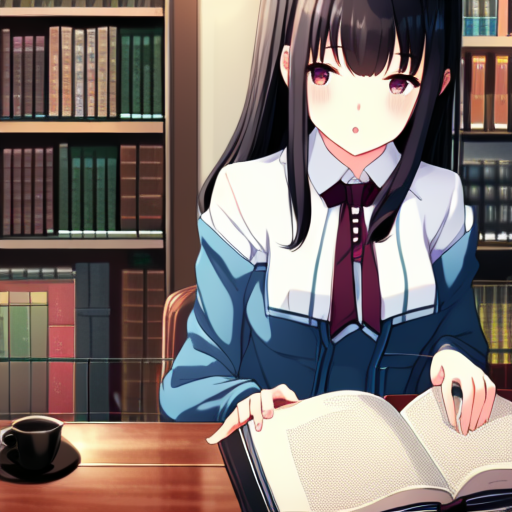
\includegraphics[scale=0.5]{./sumnail/sumnail_01.png}
      \end{center}
    \end{figure}
		%\vspace{0.5\textheight} % Whitespace between the title block and the publisher

		{\Large 量子茶房}\\[\baselineskip]% Publisher and logo

\end{titlepage}
% 標題終わり
\pagecolor{white}
\frontmatter

\tableofcontents % 目次

\mainmatter


\chapter{第一原理計算に取り組む動機}

\begin{summary}
GaNは高い破壊電界、高速な電子速度をもつことから、高周波デバイスとして広く使われており、最近では次世代パワーデバイスの開発も進んでいる。
GaNデバイスの性能向上には、結晶性、絶縁膜や金属との界面、プロセス中の表面状態など、様々な要素を改善しなくてはならない。
なかでも電気特性に大きな影響を与える電子トラップの制御が最も大きな課題の一つである。電子トラップは不純物や空孔といった結晶欠陥が原因であるが、GaNの結晶成長技術もまだ改善途上にあり詳細に調べられておらず、第一原理計算による物性予測が一歩先を行く状態である。
この章では、まずGaNの点欠陥に関する第一原理計算を行った論文とそれをもとに結晶成長条件の探索を行った論文をまとめ、第一原理計算結果の結晶成長への応用について考察する。
\end{summary}

\section{第一原理計算の結晶成長への応用}
\subsection{GaN HEMT開発における課題 電子トラップの抑制}
GaN HEMT開発における課題はいくつかあるが、その中の一つに点欠陥の抑制があげられる。
GaN中の電子トラップによって、電圧印可後に電流が減少し、時間とともに回復する現象が生じる。
高周波デバイスではこの過渡応答が信号のノイズにつながり、EVM (Error Vector Magnitude) が大きくなる。
過渡応答を抑制するためには電子トラップの抑制が不可欠だが、いったい何が原因でこの準位が形成されているのだろうか。

電子トラップの起源を調べるために数多くの実験が行われている。
様々な手法を用いて調査されており、例えばPLやCL測定で評価したGaN中のトラップ準位とその起源は次の文献にまとめられている\cite{defects_gan}。

多くは不純物元素によるものだが、なかには空孔が原因のトラップも存在しており、第一原理計算によってそのエネルギー準位が計算されている\cite{dft_gan_defect_2004},\cite{dft_gan_defect_2017}。
もちろん、不純物によってつくられるエネルギー準位も第一原理計算で計算されており、実験結果を支持するデータとして使われている。

第一原理計算は形成される欠陥の種類や欠陥準位の予測に活用されており、その計算結果を結晶成長へも応用できると考えられる。

\subsection{結晶成長への応用例}
不純物による点欠陥を抑制するための成長条件を探索するために第一原理計算を活用したという報告がある\cite{dft_gan_growth_carbon}, \cite{dft_gan_growth_oxygen}。
Reddyらは、成長中の化学ポテンシャルを変化させることでGaN中の炭素不純物を制御できたと報告し\cite{dft_gan_growth_carbon}、SzymanskiらはN極性GaN中の酸素不純物を低減したと報告している\cite{dft_gan_growth_oxygen}。

彼らは第一原理計算による点欠陥形成エネルギーと結晶成長の熱力学を結びつけるパラメータとして化学ポテンシャルに注目している。
第一原理計算での欠陥形成エネルギーの計算式に化学ポテンシャルの項が存在しており、欠陥の形成されやすさは欠陥に関係する原子の化学ポテンシャルに依存している。
成長中の各原子の化学ポテンシャルは熱力学にもとづいて炉内の原料ガスの分圧から計算することができる。
したがって、化学ポテンシャルを調整弁として点欠陥を抑制できるように成長条件を変更することが可能となる。

彼らの研究は不純物によるものだが、空孔にも応用可能と考えられる。
そこで、彼らの手法をより詳細にまとめたのち、窒素空孔抑制のための成長条件を検討する。

\subsection{第一原理計算による欠陥形成エネルギーの算出}
第一原理計算で点欠陥の形成エネルギーを計算する際には、100原子程度で構成されるスーパーセルを用いた計算がよくおこなわれている。
電荷$q$点欠陥$D$の形成エネルギーを計算する式は、
\begin{equation}
  E_{f}[D^{q}] = \qty{ E[D^{q}] + E_{\rm{corr}}[D^{q}]} - E_{P} - \sum_{i}n_{i}\mu _{i} + q\qty{ \epsilon _{\rm{VBM}}+\Delta \epsilon _{F}}
\end{equation}
とあらわされる。
ここで、$E[D^{q}]$は点欠陥を含むスーパーセルの全エネルギー, $E_{P}$は同じサイズの点欠陥を含まない完全結晶の全エネルギー, $n_{i}$は点欠陥を導入する際に追加した元素$i$の原子数(取り除いた場合は負の数になる), $\mu _{i}$は化学ポテンシャル, $\epsilon _{\rm{VBM}}$は価電子帯上端のエネルギー位置, $\Delta \epsilon _{F}$は価電子帯からのフェルミ準位のエネルギー位置を表す。
点欠陥の濃度は$10^{16} ~ 10^{20}$ cm$^{-3}$程度で物性に影響を与える。しかし、第一原理計算でこのような希薄な点欠陥を計算することは計算コストの点から不可能である。そこで、希薄極限との差分を補正するための項が$ E_{\rm{corr}}[D^{q}]$である。

第一原理計算によって計算した形成エネルギーと実際の成長条件を結び付けるにあたって、化学ポテンシャルの項に注目する。
例えば、窒素原子の位置に炭素原子が入る場合、窒素が一つ抜けて炭素が一つ結晶にはいるため、炭素と窒素の化学ポテンシャルが影響する。
窒素の化学ポテンシャルが高いと窒素が固体から抜けづらく、形成エネルギーが増加する。
Reddyらは、この予想通りに窒素の化学ポテンシャルを上げると、炭素濃度が減少すると報告している。

では、窒素空孔の場合はどうだろうか。
数式を書くと、
\begin{equation}
  E_{f}[V_{N}^{q}] = \qty{ E[V_{N}^{q}] + E_{\rm{corr}}[V_{N}^{q}]} - E_{P} + \mu _{N} + q\qty{ \epsilon _{\rm{VBM}}+\Delta \epsilon _{F}}
\end{equation}
となる。
窒素空孔も窒素が固体から抜けづらくすればよいので、窒素の化学ポテンシャルを上げることで形成エネルギーがあがり、窒素空孔が減少すると考えられる。

\subsection{化学ポテンシャルと成長条件の関係}
先ほどの節でみたように化学ポテンシャルによって点欠陥の形成エネルギーが変化することから、成長条件によって化学ポテンシャルを制御すれば点欠陥の形成を制御できると考えられる。

化学ポテンシャルは原料ガスの分圧から求められる。
結晶成長中のGaN表面におけるGaの化学ポテンシャルはGaの標準状態(金属Ga)と等しく、
\begin{equation}
  \mu_{\rm{Ga}} = kT \log \qty(\frac{P_{eq}^{\rm{Ga}}}{P_{V}^{\rm{Ga}}})
\end{equation}
とあらわせる。
ここで、$P_{eq}^{\rm{Ga}}$は成長中のGaN表面におけるGaの平衡分圧, $P_{V}^{\rm{Ga}}$は成長温度における金属Gaの平行蒸気圧をあらわす。
したがって、成長条件に対してGaの平衡分圧を計算することができれば、化学ポテンシャルを計算することが可能となる。

さらに、GaとNの平衡状態における化学ポテンシャルは次のような関係をもつ。
\begin{align}
  \mu_{\rm{Ga}} + \mu_{\rm{N}} = \mu_{\rm{GaN}} \\
  \mu_{\rm{GaN}} = \mu_{\rm{Ga}_{l}} + 0.5  \mu_{\rm{N}_{2}} + \Delta H_{f}
\end{align}
ここで、$\mu_{\rm{GaN}}$と$\Delta H_{f}$はGaNの化学ポテンシャルと生成エンタルピーをあらわす。
また、基準とする状態からのGaの化学ポテンシャルの変化、$\Delta \mu_{\rm{Ga}}$はNの化学ポテンシャルの変化と関係があり、

となる。
したがって、ある成長条件におけるGaの平衡分圧をもとめれば、Gaの化学ポテンシャルの変化と同時にNの化学ポテンシャルの変化も計算することが可能となる。
\begin{align}
  \Delta \mu_{\rm{Ga}} + \Delta \mu_{\rm{N}} = 0 \\
  \Delta \mu_{\rm{N}} = - \Delta \mu_{\rm{Ga}}
\end{align}
\subsection{GaN MOCVD成長における平衡分圧の計算}
GaN MOCVD成長時の原料の平衡分圧は熱力学を使って計算することができる。
詳細は纐纈らによって報告されており\cite{movpe_gan}, \cite{movpe_gan_jap}、ここではGaNの成長について紹介する。

平衡分圧を計算するにあたって、いくつかの仮定をおこなう。
まず最初の仮定は、MOCVD成長の成長速度はIII族原料の物質輸送律速であるという仮定である。
この仮定のもとでは化学反応速度は原料の到達速度よりも早いため、気相-固相の間で化学平衡が成り立つと仮定することができる。

また、トリメチルガリウム(TMGa)とNH$_{3}$を原料とするGaNの成長を考え、供給された有機金属原料は気相-固相界面で不可逆的に分解し、
\begin{equation}
  \rm{Ga(CH}_{3}\rm{)}_{3}(\rm{g}) + \frac{3}{2}\rm{H}_{2}(\rm{g}) \rightarrow \rm{Ga}(\rm{g}) + 3\rm{CH}_{4}(\rm{g})
\end{equation}
となっていると仮定する。

GaNの成長に関与する分子種はGa, NH$_{3}$, H$_{2}$, 炭化水素(CH$_{4}$), 不活性ガス(N$_{2}$)である。
気相-固相界面におけるGaNの成長反応は、
\begin{equation}
  \rm{Ga}(\rm{g}) + \rm{NH}_{3}(\rm{g}) = \rm{GaN}(\rm{s}) + \frac{3}{2}\rm{H}_{2}(\rm{g})
\end{equation}
とあらわされる。
この式に対する質量作用の法則より、
\begin{equation}
  K = \frac{a_{\rm{GaN}}P_{\rm{H}_{2}}^{3/2}}{P_{\rm{Ga}}\cdot P_{\rm{NH}_{3}}}
\end{equation}
が成り立つ。
また、系の全圧から、
\begin{equation}
  \sum P = P_{\rm{Ga}}+P_{\rm{NH}_{3}} + P_{\rm{H}_{2}} + P_{\rm{N}_{2}} + P_{\rm{CH}_{4}}
\end{equation}
となり、系の束縛条件から、
\begin{align}
  P_{\rm{Ga}}^{in}- P_{\rm{Ga}} &= P_{\rm{NH}_{3}}^{in} - P_{\rm{NH}_{3}} \\
  P_{\rm{CH}_{4}} &= 3 P_{\rm{Ga}} \\
  F &= P_{\rm{H}_{2}} / (P_{\rm{H}_{2}} + P_{\rm{N}_{2}})
\end{align}
となる。ここで、$P_{i}^{in}$は$i$の供給分圧を示し、$P_{i}$は平衡分圧を示す。

NH$_{3}$は300℃以上の温度では熱分解するが、触媒のない通常の成長条件のもとでは分解速度は遅い。そのため、NH$_{3}$の分解率$\alpha$を導入し、成長表面に到達するNH$_{3}$を計算する。
\begin{equation}
  \rm{NH}_{3}(\rm{g}) \rightarrow (1-\alpha ) \rm{NH}_{3}(\rm{g}) + \frac{\alpha}{2} \rm{N}_{2}(\rm{g}) + \frac{3\alpha}{2} \rm{H}_{2}(\rm{g})
\end{equation}

以上の式(1.10)~(1.14)を連立させて解くことで、各原料の平衡分圧を計算することが可能であり、その計算結果を活用して化学ポテンシャルの変化を予想することができる。

\subsection{まとめ}
第一原理計算から点欠陥の形成エネルギーを求めることが可能で、そのエネルギーは欠陥形成にかかわる原子の化学ポテンシャルに依存する。
成長条件における化学ポテンシャルは熱力学に基づいて計算することが可能である。
したがって、熱力学を使って計算した化学ポテンシャルの値を第一原理計算に活用することで、点欠陥の形成を抑制できる成長条件の探索が可能になると考えられる。
次章から、第一原理計算のやり方についてまとめていく。

\chapter{構造最適化計算}

\begin{summary}
第一原理計算は、 物質や構造の特性を理解するための重要なツールである。しかし、計算を行う前には、研究対象となる系の構造を最適化することが非常に重要である。なぜなら、構造中の原子の配置が不自然だと、計算で得られる結果がどうしても正しくなくなるからである。構造を最適化し、安定な原子配置に基づいて計算を行うことは、第一原理計算で得られる結果の精度を保証するための重要なステップである。構造の最適化では、系が最小エネルギーの状態に達するまで、格子内の原子の位置を調整する。計算の結果得られた原子配置は、最も安定した原子配置\footnote{計算の結果得られた構造が局所安定な解であることは確認する必要がある。また、構造最適化だけでは不十分な場合もある。}であり、今後の第一原理計算の良い出発点となる。
\end{summary}

\newpage

\section{構造最適化計算のやり方}
Quantum Espressoでおこなえる構造最適化計算は次の二種類がある。
\begin{enumerate}
  \item 格子定数は変化させずに、原子の内部座標を最適化する。
  \item 内部座標とともに格子定数も変化させて最適化する。
\end{enumerate}

webサイト\cite{qe-tutorial_kyoto-yukawa}からSiの構造緩和計算を行う計算例を引用し示したのち、それを参考に作成したGaNの構造最適化計算の例を示す。

\section{Siの構造最適化}
\subsection{原子位置の構造緩和}
Siの格子定数はそのままで、構造緩和させる。
本来、単位胞内におけるSi原子の位置は(0, 0, 0)と(0.25, 0.25, 0.25)であるが、わざと少しずらした点で構造緩和させてみる。
\begin{example}{Si.relax.in}
\begin{verbatim}
  &control
     calculation='relax'
     prefix='Si'
     pseudo_dir='./pseudo/'
     outdir = './tmp/'
     etot_conv_thr = 1.d-5
     forc_conv_thr = 1.d-4
  /
  &system
     ibrav=  2, celldm(1) =10.2, nat=  2, ntyp= 1,
     ecutwfc = 30.0,
  /
  &electrons
     conv_thr = 1.0d-8
  /
  &ions
  /
  ATOMIC_SPECIES
   Si  28.086  Si.pz-vbc.UPF
  ATOMIC_POSITIONS
   Si 0.00 0.00 0.00 0 0 0
   Si 0.22 0.23 0.24
  K_POINTS automatic
    6 6 6 1 1 1
\end{verbatim}
\end{example}
入力パラメータのうち構造緩和に関係するところを説明する。
まず、格子定数を変化させない場合は、calculation='relax'とする。
構造緩和における収束の判断を行う閾値は、\verb|etot_conv_thrとforc_conv_thr|である。前者はエネルギーの変化に関する閾値、後者は原子に加わる力の変化に関する閾値である。

加えて、relax計算の場合、\verb|&|ionsという項目が必要となる。上記ではこの項目はデフォルトの値を使用している。

原子位置に関して、原点のSi原子は動かしたくないため、座標の後ろに0 0 0を付け加えている。これは第一成分、第二成分、第三成分のすべてを動かさないという記述で、例えば第一成分のみ動かしたい場合は1 0 0を付け加える。

\subsection{格子定数の構造緩和}

続いて、格子定数の構造緩和を行う例を示す。
Siの格子定数はボーア半径単位で10.2程度であり、少しずらして構造緩和を行う。

先ほどのSi.relax.inとの違いは、
\begin{itemize}
  \item calculation='vc-relax'に変更
  \item \verb|&|cellを追加
  \item \verb|press_conv_thr|を追加(任意)
\end{itemize}
である。

\begin{example}{Si.vc-relax.in}
\begin{verbatim}
  &control
     calculation='vc-relax'
     prefix='Si'
     pseudo_dir='./pseudo/'
     outdir = './tmp/'
     etot_conv_thr = 1.d-5
     forc_conv_thr = 1.d-4
  /
  &system
     ibrav=  2, celldm(1) =10.0, nat=  2, ntyp= 1,
     ecutwfc = 30.0,
  /
  &electrons
     conv_thr = 1.0d-8
  /
  &ions
  /
  &cell
    press_conv_thr = 0.1
  /
  ATOMIC_SPECIES
   Si  28.086  Si.pz-vbc.UPF
  ATOMIC_POSITIONS
   Si 0.00 0.00 0.00 0 0 0
   Si 0.25 0.25 0.25
  K_POINTS automatic
    6 6 6 1 1 1
\end{verbatim}
\end{example}

\section{GaNの構造最適化}
Si原子の入力ファイル例を参考に、GaNの構造緩和計算のための入力ファイルを作成する。
\subsection{原子位置の構造緩和}
格子定数はそのままに、原子位置の構造緩和をおこなう。
入力ファイルは下記の通りである。
\begin{example}{GaN.relax.in}
\begin{verbatim}
  &control
      calculation='relax' ,
      restart_mode='from_scratch' ,
      prefix='GaN' ,
      outdir = './GaN/' ,
      wfcdir = './GaN/' ,
      pseudo_dir = './PP' ,
      disk_io='default' ,
      forc_conv_thr= 1.d-4 ,
      etot_conv_thr= 1.d-5 ,
      verbosity = 'high' ,
      nstep = 200 ,
   /
   &system
      ibrav= 4 ,
      celldm(1) = 6.02822634 ,
      celldm(3) = 1.62664576803 ,
      nat =  4 ,
      ntyp = 2 ,
      ecutwfc = 60.0 ,
      ecutrho = 360.0 ,
      nosym = .true.
   /
   &electrons
      electron_maxstep = 200 ,
      mixing_beta = 0.7 ,
  !   use smaller conv_thr for better results ,
      conv_thr = 1.0d-14 ,
   /
   &ions
   /
  ATOMIC_SPECIES
  Ga     69.72300  Ga.pbe-dnl-rrkjus_psl.1.0.0.UPF
  N      14.00674  N.pbe-n-rrkjus_psl.1.0.0.UPF
  ATOMIC_POSITIONS crystal
  Ga     0.666667   0.333333   0.000000 1 1 0
  Ga     0.333333   0.666667   0.500000
  N      0.666667   0.333333   0.375000
  N      0.333333   0.666667   0.875000
  K_POINTS automatic
   7 7 4 1 1 1
\end{verbatim}
\end{example}
Siの場合と違って(0, 0, 0)の原点に原子は存在せず、(2/3, 1/3, 0)にGa原子が存在している。そこで、第三成分のみ固定し、原子位置の構造緩和計算を実施している。
GaNの単位胞はc軸 = z方向に長い格子なので、k点の切り方もz方向はx, y方向の半分に設定している。

\subsection{格子定数の構造緩和}
続いて、格子定数の構造緩和の入力ファイル例を示す。
原子位置は上記の原子位置の構造緩和によって得られた結果を反映している。
\begin{example}{GaN.vc-relax.in}
\begin{verbatim}
  &control
      calculation='vc-relax' ,
      restart_mode='from_scratch' ,
      prefix='gan_wz' ,
      outdir = './gan_wz/' ,
      wfcdir = './gan_wz/' ,
      pseudo_dir = './PP' ,
      disk_io='default' ,
      forc_conv_thr= 1.d-4 ,
      etot_conv_thr= 1.d-5 ,
      verbosity = 'high' ,
      nstep = 200 ,
   /
   &system
      ibrav= 4 ,
      celldm(1) = 6.02822634 ,
      celldm(3) = 1.62664576803 ,
      nat =  4 ,
      ntyp = 2 ,
      ecutwfc = 60.0 ,
      ecutrho = 360.0 ,
      nosym = .true.
   /
   &electrons
      electron_maxstep = 200 ,
      mixing_beta = 0.7 ,
  !   use smaller conv_thr for better results ,
      conv_thr = 1.0d-14 ,
   /
   &ions
      ion_dynamics='bfgs' ,
   /
   &cell
      press_conv_thr = 0.1
   /
  ATOMIC_SPECIES
  Ga     69.72300  Ga.pbe-dnl-rrkjus_psl.1.0.0.UPF
  N      14.00674  N.pbe-n-rrkjus_psl.1.0.0.UPF
  ATOMIC_POSITIONS crystal
  Ga 0.6666619112 0.3333380861 0.0000000000 1 1 0
  Ga 0.3333380928 0.6666619098 0.5000041533
  N  0.6666761483 0.3333238540 0.3769034997
  N  0.3333238477 0.6666761500 0.8768910442
  K_POINTS automatic
   7 7 4 1 1 1
\end{verbatim}
\end{example}

\subsection{構造最適化の結果}
上記の入力ファイルで構造最適化計算を行った結果は表\ref{gan_str-opt}に示す。
初期の値は実験で得られた格子定数で、最適化後にはa軸とc軸どちらも実験値より大きな値となった。

\begin{table}[hbt]
  \caption{GaNの構造最適化計算の結果}
  \label{gan_str-opt}
  \centering
  \begin{tabular}{lccc}
    \hline
     & a [$\AA$] & c [$\AA$] & a/c \\
     \hline \hline
     初期 & 3.19 & 5.189 & 1.627 \\
     最適化後 & 3.215 & 5.239 & 1.629\\
     \hline
  \end{tabular}
\end{table}

上記の結果について、論文で報告されている結果と比較してみる。GaNの構造最適化計算に関する論文\cite{GaN_DFT_str}で述べられている結果を表\ref{gan_str-opt-ref}に示す。

\begin{table}[hbt]
  \caption{論文で報告されているGaNの構造最適化結果\cite{GaN_DFT_str}}
  \label{gan_str-opt-ref}
  \centering
  \begin{tabular}{lccc}
    \hline
     & a [$\AA$] & c [$\AA$] & a/c \\
     \hline \hline
     LDA & 3.196 & 5.213 & 1.631 \\
     PBE & 3.252 & 5.298 & 1.629\\
     Exp.\cite{GaN_DFT_str_2} & 3.189 & 5.179 & 1.624\\
     \hline
  \end{tabular}
\end{table}

論文ではLDAとPBE(GGA)で計算した場合の結果を比較しており、交換相関項の違いで構造最適化後の格子定数に違いがみられる。

今回の計算はPBEを用いて計算しており、論文と同程度の結果が得られていることがわかる。このことから、上記の入力ファイルで問題なく計算が実行できていると判断した。

\section{構造最適化に関するトピック}
\subsection{得られる格子定数の結果に関して}
一般的に構造最適化で得られる格子定数は、LDA計算(PZ型の擬ポテンシャルなど)では過小評価され、GGA計算(PBE型の擬ポテンシャルなど)では過大評価される。

最近ではPBEを改善したPBESOLという交換相関ポテンシャルが実験の格子定数を比較的よく再現できるようになっている。しかし、格子定数を計算から求めるのは困難なので、実運用上は格子定数は測定値を使用し、内部座標についてのみ最適化を行うことが多い。
\section{まとめ}

\chapter{電子状態の計算}
\begin{summary}
第一原理計算は、物質中の電子の波動関数を密度半関数法を用いて計算している。この計算には、自己無撞着計算が必要であり、反復計算を行うことで十分に収束した波動関数が得られる。得られた波動関数は、電子状態密度やバンド分散など、さまざまな電子状態の物理量を計算するために使用することができる。この章では、自己無撞着計算やその結果を利用した電子状態密度やバンド分散の計算方法を説明する。
\end{summary}

\newpage

\section{自己無撞着計算}
自己無撞着計算(Self-consistent Field, SCF)計算を行うための入力ファイルを作成する。
GaNのSCF計算の入力ファイルは下記のとおりである。
入力ファイルの作成、計算結果の確認は文献\cite{maezono_DFT}を参考におこなった。

\begin{example}{GaN.scf.in}
\begin{verbatim}
  &control
    calculation = 'scf'
    restart_mode = 'from_scratch'
    prefix = 'gan'
    outdir = 'out_gan'
    pseudo_dir = './PP'
  /
  &system
    ibrav = 4
    a = 3.2153
    c = 5.23899
    nat = 4
    ntyp = 2
    occupations = 'fixed'
    ecutwfc = 50
    ecutrho = 400
    nbnd = 20 !18 filled bands, 2 more empty bands
  /
  &electrons
  /
  K_POINTS {automatic}
  2 2 2 1 1 1
  ATOMIC_SPECIES
    Ga   69.72300  Ga.pbe-dn-kjpaw_psl.1.0.0.UPF
     N   14.00650  N.pbe-n-kjpaw_psl.1.0.0.UPF
  ATOMIC_POSITIONS {crystal}
  Ga 0.6666680851 0.3333319134 0.0000000000
  Ga 0.3333319519 0.6666680855 0.5000260061
  N  0.6666925477 0.3333074525 0.3766951515
  N  0.3333074513 0.6666925484 0.8767004581
\end{verbatim}
\end{example}
原子位置は第2章で計算した構造最適化の結果を利用している。

自己無撞着計算が終わったら、正しく計算が行われているのか確認する。
計算結果であるscf.outからtotal energyの項を次のようなコマンドで確認する。
\begin{code}
\begin{verbatim}
  grep 'total energy ' scf.out
\end{verbatim}
\end{code}
上記のコマンドを実行すると下記のようにtotal energyの値が表示される。
\begin{code}
\begin{verbatim}
  total energy              =    -611.70547437 Ry
  total energy              =    -612.17226092 Ry
  total energy              =    -612.41317647 Ry
  ...
  total energy              =    -612.45360188 Ry
  total energy              =    -612.45360152 Ry
! total energy              =    -612.45360151 Ry
\end{verbatim}
\end{code}
自己無撞着計算のイタレーションの過程におけるtotal energyが表示されており、次第に収束していっていることが確認できる。
エネルギーが十分に収束していなくても、イタレーション回数の上限に達すると計算が終了するため、まずは収束しているかどうかを確認することが重要である。
計算が収束していることを確認出来たら、次は状態密度の計算を行う。
\section{状態密度の計算}
状態密度の計算は先ほど自己無撞着計算で得られた電子状態を用いて行う。ここでは、自己矛盾な状態に十分収束した結果を使うので、SCFループを回す必要はない。
収束し終えた結果を使って計算することから、non-SCFという意味で、NSCF計算と呼ぶ。

\subsection{NSCF計算}
先ほどのGaNのSCF計算に使用したインプットファイルをコピーして、NSCF計算用に次のように書き換える。
\begin{example}{GaN.nscf.dos.in}
\begin{verbatim}
  &control
  calculation = 'nscf'
  restart_mode = 'from_scratch'
  prefix = 'gan'
  outdir = 'out_gan'
  pseudo_dir = './PP'
/
&system
  ibrav = 4
  a = 3.21374
  c = 5.23521
  nat = 4
  ntyp = 2
  occupations = 'tetrahedra'
  ecutwfc = 50
  ecutrho = 400
  nbnd = 20 ! 18 filled bands , 2 more empty bands
/
&electrons
/
K_POINTS {automatic}
4 4 2 0 0 0
ATOMIC_SPECIES
  Ga   69.72300  Ga.pbe-dn-kjpaw_psl.1.0.0.UPF
   N   14.00650  N.pbe-n-kjpaw_psl.1.0.0.UPF
   ATOMIC_POSITIONS {crystal}
   Ga 0.6666680851 0.3333319134 0.0000000000
   Ga 0.3333319519 0.6666680855 0.5000260061
   N  0.6666925477 0.3333074525 0.3766951515
   N  0.3333074513 0.6666925484 0.8767004581
\end{verbatim}
\end{example}
まず、calculation='nscf'とし、NSCF計算に切り替える。
次に、outdirをSCF計算で得られたデータが格納されているディレクトリを選択する。端的に言えば、SCF計算と同じディレクトリを指定する。

続いて、occupation = 'tetrahedra'を選択する。
こうすることで、テトラヘドロン法(四面体法)
を使ってブリルアンゾーン内のk点の積分が実行される。
テトラヘドロン法はブリルアンゾーン内を多数の四面体で区切り、その四面体内でフェルミエネルギーまでの状態(体積)を線形補間などで解析的に足し上げる。これを改良する方法としてBlochl補正\cite{Blochl}が知られており、Quantum Espressoではこれを利用している。

\subsection{状態密度の描画}
NSCF計算が終了したら、状態密度(Density of States)を計算するための入力ファイル、dos.inを用意する。
\begin{example}{dos.in}
\begin{verbatim}
&dos
outdir = './out_gan',
prefix='gan',
fildos='gan.dos',
/
\end{verbatim}
\end{example}
DOSの計算時にはpw.xではなく、dos.xを使用する。
上記の計算を実行すると、gan.dosという出力ファイルにDOSの描画に必要となるデータが出力される。

\begin{code}
\begin{verbatim}
  #  E (eV)   dos(E)    Int dos(E) EFermi =  10.744 eV
    -6.475  0.0000E+00  0.0000E+00
    -6.465  0.4054E-03  0.1351E-05
    -6.455  0.1621E-02  0.1081E-04
    -6.445  0.3648E-02  0.3648E-04
    -6.435  0.6486E-02  0.8647E-04
    -6.425  0.1013E-01  0.1689E-03
    ...
\end{verbatim}
\end{code}
1列目がプロットの横軸となるエネルギー、2列目が状態密度である。3列目は状態密度を積分した値で、そのエネルギーいかにどれだけの状態が存在するかに相当する値である。
このデータを使ってgnuplot等でグラフにすることで状態密度のグラフを描画することができる。

\subsection{部分状態密度の描画}
部分状態密度(partial DOS)とは、状態密度を各軌道成分に分解して、それらの寄与を図示したものである。
DOSの計算時にはdos.xを使用したが、projwfc.x\footnote{各成分に射影するという意味のprojectionと波動関数のwavefunctionを組み合わせたニーモニックである。}を使用する。
projwfc.xで実行する入力ファイルpdos.inは次のとおりである。
\begin{example}{pdos.in}
\begin{verbatim}
&projwfc
outdir = './out_gan',
prefix='gan',
degauss=0.01,
/
\end{verbatim}
\end{example}

degaussというパラメータについて説明する。
計算上、有限個のk点を用いて計算しているため、状態密度のグラフはガタガタになってしまう。このガタガタに対してアンチエイリアス処理を施して精度の向上を図っている。
いくつか方法があるが、カウス関数を使ってアンチエイリアス処理が行われており、使用するガウス関数の幅をdegaussで設定する。
degaussの単位はRyで、値としては0から数Ry程度に設定することが一般的である\cite{SCF_example_qiita}。

上記のファイルを実行すると、ディレクトリ内に各原子の各軌道(s, p, d, ...)のpDOSが出力される。
これらを描画することで、部分状態密度の図を描くことができる。

\section{バンド分散の計算}
バンド分散の計算では、描画するバンド本数とk点パスを指定する必要がある。

バンド本数は価電子帯に加えて伝導帯を何本まで描画するか、を指定する。原理的には高エネルギー側に向かって無限本のバンドが存在するため、どこまで計算するか指定する必要がある。

k点パスについて説明する。エネルギーバンドは各バンドの固有値のkベクトルに対する依存性を描画した図である。ブリルアンゾーン内の三次元k空間上の各点に対する各バンドのエネルギーを計算されるが、これを二次元の図におとした図がエネルギーバンド図である。二次元の図としてあらわす際に、三次元のk空間中を走る特徴的な経路(一次元)をとってその経路に沿って各バンドのエネルギーがどのように変化するかを図示する。
この一次元の特徴的な経路をk点パスと呼ぶ。
対象とする結晶構造ごとに標準的なk点パスが決まっており、それに従って計算する。

実際にバンド分散を計算する手順について説明する。

\subsection{NSCF計算}
まずは描画するバンドの本数を決定する。
SCF計算の出力ファイル、scf.outに単位胞内の電子数が記入されており、それを次のようなコマンドで取得する。
\begin{code}
\begin{verbatim}
  grep 'number of electrons' scf.out
  number of electrons = 36.00
\end{verbatim}
\end{code}
単位胞内の電子が36個ということは、一つの準位にスピンが上向きと下向きの2つの電子が占有するので、18番目までのバンドが占有されていることになる。

伝導帯(非占有バンド)としては占有バンドの本数の半分程度までを描画すれば十分と考え、計算するバンドの本数は27本とする。

状態密度を計算するときに使用したNSCF計算用のインプットファイルを次のように書き換える。

\begin{example}{GaN.nscf.disp.in}
\begin{verbatim}
&control
  calculation = 'bands'
  restart_mode = 'from_scratch'
  prefix = 'gan'
  outdir = 'out_gan'
  pseudo_dir = './PP'
/
&system
  ibrav = 4
  a = 3.21374
  c = 5.23521
  nat = 4
  ntyp = 2
  occupations = 'fixed'
  ecutwfc = 80
  ecutrho = 720
  nbnd = 27 ! 18 filled bands , 9 more empty bands
/
&electrons
 conv_thr = 1.00000e-08
 diago_david_ndim = 4
/
K_POINTS {crystal_b}
12
0.0 0.0 0.0 20
0.5 0.0 0.0 20
0.333333333333333 0.333333333333333 0.0 20
0.0 0.0 0.0 20
0.0 0.0 0.5 20
0.5 0.0 0.5 20
0.333333333333333 0.333333333333333 0.5 20
0.0 0.0 0.5 20
0.5 0.0 0.5 20
0.5 0.0 0.0 20
0.333333333333333 0.333333333333333 0.0 20
0.333333333333333 0.333333333333333 0.5 20

ATOMIC_SPECIES
  Ga   69.72300  Ga.pbe-dn-kjpaw_psl.1.0.0.UPF
   N   14.00650  N.pbe-n-kjpaw_psl.1.0.0.UPF
ATOMIC_POSITIONS {crystal}
Ga  0.6666680851 0.3333319134 0.0000000000
Ga  0.3333319519 0.6666680855 0.5000260061
N   0.6666925477 0.3333074525 0.3766951515
N   0.3333074513 0.6666925484 0.8767004581
\end{verbatim}
\end{example}
入力パラメータのうち、nbndが計算するバンドの本数、\verb|K_POINTS|で指定しているk点が六方晶のk点パスである。
k点パスの詳細は別の節で詳しく説明する。

\subsection{バンド分散図の描画}
上記のNSCF計算を実行することで、指定したk点でのエネルギー固有値が計算される。
その計算結果に基づいて、bands.xで分散図の出力を行う。
bands.xの入力ファイルは次のとおりである。
\begin{example}{bands.in}
\begin{verbatim}
  &bands
  outdir = './out_gan',
  prefix='gan',
  filband='gan.band',
  lsym=.true.
  /
\end{verbatim}
\end{example}
これを実行すると、gan.band, gan.band.gnu, gan.band.rapの3つのファイルが作成される。
まずは、gan.bandを使って分散図を描画する。

バンド図の可視化はplotband.xを使うことで行える。
plotband.xを実行するとxmgr形式とps形式の二つのファイルが生成される。
xmgr形式のファイルはGraceというソフトで図を作成するためのファイルで、本格的な図を作成する場合に使うものである。
バンド分散図を作成して計算がうまくいっているかどうか確認する程度であれば、ps形式で問題ない。

plotband.xでは、表示範囲、SCF計算で得られたフェルミ準位の値、プロットの目盛り幅などを指定する。
今回は、以下のように作成した。
\begin{example}{plotband.in}
\begin{verbatim}
  gan.band !対象のファイル
  0 14 !表示範囲
  gan.band.xmgr !xmgr形式の出力ファイル名
  gan.band.ps !ps形式の出力ファイル名
  10.7445 !フェルミ準位のエネルギー値
  1 10.7445 !縦軸の目盛り幅、フェルミ準位のエネルギー
\end{verbatim}
\end{example}
表示範囲は絶対値で指定するが、グラフはフェルミ準位のエネルギーが0になるように縦軸を変換しているため、図\ref{fig_plotband}のようなグラフになる。
もう少し表示範囲を高エネルギー側にずらせば、見やすい図になる。(今回は値の設定の仕方を見せるためにわざとずらしている。)

\begin{figure}[bht]
  \centering
  \includegraphics[scale=0.35,bb=0 0 612 792, angle=270]{./chap03/gan.band.eps}
  \caption{plotband.xで作成したバンド分散図}
  \label{fig_plotband}
\end{figure}

続いて、gnuplotを使ってグラフを描画する例を示す。
gnuplotでデータを書くときには、bands.xで得られたgan.band.gnuを使う。
gnuplotでバンド分散図を描く場合は、次のようなpltファイルを用意する。

\begin{example}{band.plt}
\begin{verbatim}
unset key
set grid xtics

G1 = 0.0000
M = 0.5774
K = 0.9107
G2 = 1.5774
A = 1.8842
L = 2.4616
H = 2.7949
A2 = 3.4616
L2 = 4.0389
M2 = 4.3458
K2 = 4.6791
H2 = 4.9860

set xtics ("{/Symbol G}" G1, "{M}" M, "{K}" K, \
"{/Symbol G}" G2, "{A}" A, "{L}" L, "{H}" H, \
 "{A}" A2, "{L}" L2, "{M}" M2, "{K}" K2, "{H}" H2)

set ylabel "Energy [eV]" font "Arial, 14"
set yrange [-5:9]

VBM = 9.27013 #Valence band Maximum [eV]

plot "gan.band.gnu" u 1:($2-VBM) w l lw 1.5 lc "red",\
0 w l lc "black" dt (10, 10)
\end{verbatim}
\end{example}
上のファイルを実行して得られた図を図\ref{fig_gnuplot}に示す。

\begin{figure}[htb]
  \centering
  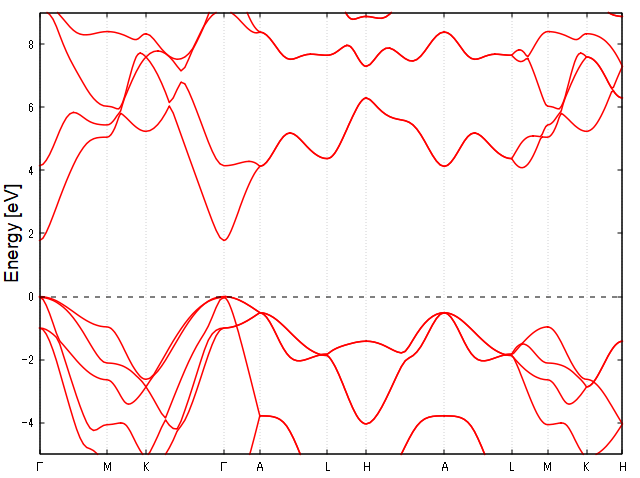
\includegraphics[scale=0.5]{./chap03/GaN_band.png}
  \caption{gnuplotで作成したバンド分散図}
  \label{fig_gnuplot}
\end{figure}
gnuplotのほうが入力パラメータは多いが、グラフの自由度は高い。
また、pltファイルを一度作成すれば、使いまわすことができるので、
二回目以降はそれほど手間がかからないこともメリットである。

\subsection{k点パス}

\bibliographystyle{unsrt}
\bibliography{./ref/export.bib}



\backmatter
\printindex

\end{document}
